\newpage
\section{Precio de talleres y combustible}
\label{anexo_precio_taller_combustible}

Una motocicleta necesita un mantenimiento cada cierto tiempo o kilometraje, al año se estima que se necesitan los mantenimientos de la \autoref{tabla: reparaciones y precios} y su coste.

\begin{table}[H]
\centering
\begin{tabular}{|c|c|c|}
\hline
                           & \textbf{Nº veces/año} & \textbf{Coste total (\glssymbol{euro})} \\ \hline
\textbf{Cambios de aceite} & 1                     & 80                   \\ \hline
\textbf{Revisiones}        & 0,33                  & 66                   \\ \hline
\textbf{Ruedas}            & 0,5                   & 40                   \\ \hline
\textbf{Frenos}            & 0,5                   & 20                   \\ \hline
\textbf{Transmisión}       & 0,33                  & 33                   \\ \hline
\textbf{TOTAL}             &                       & \textbf{239}                 \\ \hline
\end{tabular}
\caption{Reparaciones y precios de motocicletas y ciclomotores.}
\label{tabla: reparaciones y precios}
\end{table}

El mantenimiento de las motos eléctricas no resulta tan caro en comparación a las de gasolina, resultando en 126 \glssymbol{euro}.

El mantenimiento de un patinete es más económico, tal y como se observa en la \autoref{tab: Reparaciones y precios patinetes} \cite{tarifaspatinete1}, considerando que tiene componentes electrónicos que pueden hacer más elevado su precio.

\begin{table}[H]
\centering
\begin{tabular}{|l|l|}
\hline
\textbf{}                               & \multicolumn{1}{c|}{\textbf{Precio (\glssymbol{euro})}} \\ \hline
\textbf{Cambio de 2 ruedas 10 pulgadas} & 25                                  \\ \hline
\textbf{Luces, acelarador, dirección}   & 8,95                                  \\ \hline
\textbf{Ajuste de frenos}               & 15,95                                 \\ \hline
\textbf{Cambio de batería}              & 34,95                                 \\ \hline
\textbf{Suspensión}                     & 39,95                                 \\ \hline
\textbf{Total}                          & \textbf{124,8}                       \\ \hline
\end{tabular}
\caption{Reparaciones y precios de patinetes.}
\label{tab: Reparaciones y precios patinetes}
\end{table}


Para garantizar tener capital de respaldo para sustituir un vehículo entero en caso de siniestro, se le suman a los patinetes y a las motos un respaldo que permitan ahorrar para su sustitución, de 20 \gls{euro} y 100 \gls{euro} anuales por vehículo respectivamente.


Por otro lado, el valor del precio de la electricidad y gasolina se ha obtenido mediante los datos diarios del año anterior al presente \cite{historicoluz,historicocombustible}. Sus representaciones gráficas sobre la fluctuación de mercado, tal y como se muestran en la \autoref{fig:precio luz 2021} y \autoref{fig:precio gasolina 2021}, siendo el precio medio de la gasolina de 1,38 \glssymbol{euro}/\glssymbol{litros}, y el de la luz de 111,93 \glssymbol{euro}/MWh.

\begin{figure}[H]
    \centering
    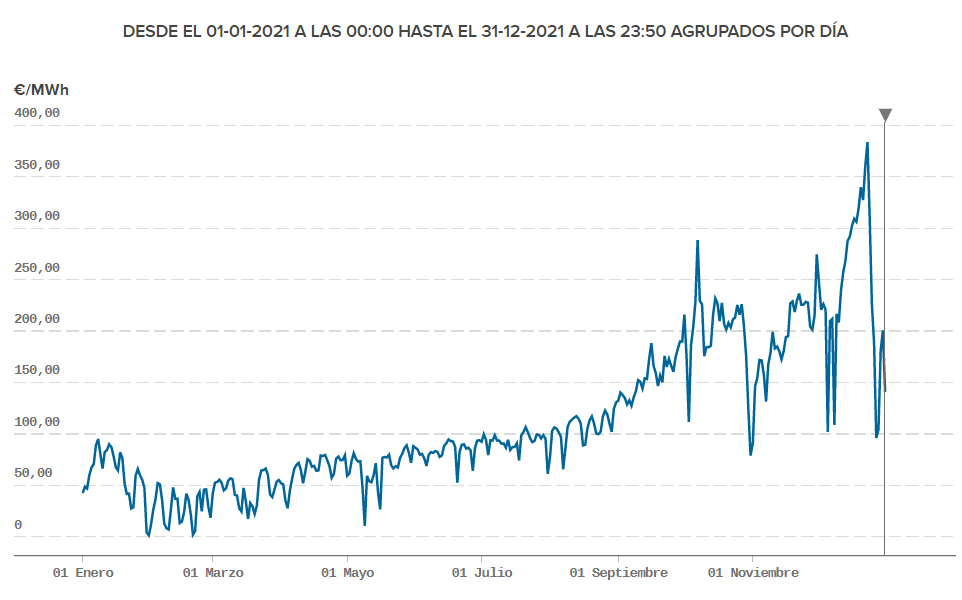
\includegraphics[scale=0.4]{archivos/precio luz 2021.png}
    \caption{Histórico precio electricidad.}
    \label{fig:precio luz 2021}
\end{figure}

\begin{figure}[H]
    \centering
    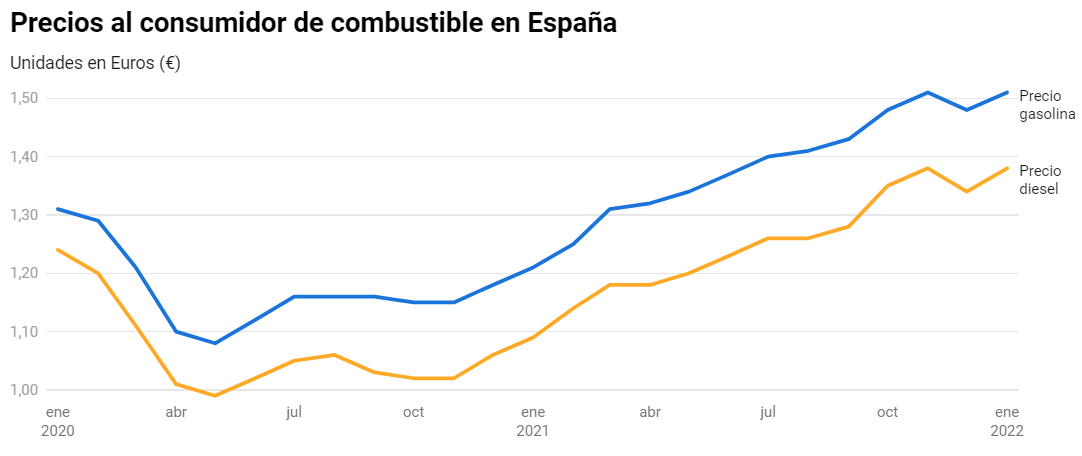
\includegraphics[scale=0.35]{archivos/precio gasolina 2021.png}
    \caption{Histórico precio combustible.}
    \label{fig:precio gasolina 2021}
\end{figure}

\newpage
% \addcontentsline{toc}{section}{Referencias}
% \section*{Referencias}
% \label{referencias_nucleo}
% \makeatletter
% \def\@bibitem#1{\item\if@filesw \immediate\write\@auxout
%   {\string\bibcite{#1}{A\the\value{\@listctr}}}\fi\ignorespaces}
% \def\@biblabel#1{[A{#1}]}
% \makeatother
% \printbibheading[title={Referencias},heading=bibintoc]
\nocite{*}
\newrefcontext[labelprefix=\thesection.]
\printbibheading[title={Referencias},heading=subbibintoc]
\printbibliography[heading=none,resetnumbers=true,keyword=preciotaller]